\documentclass[12pt,a4paper]{article}
\usepackage[utf8]{inputenc}
\usepackage{amsmath}
\usepackage{verbatimbox}
\usepackage{xcolor}
\usepackage{hyperref}

\usepackage{listings}
\lstset{
    basicstyle=\ttfamily,
    columns=flexible,
    breaklines=true,
    postbreak=\mbox{\textcolor{red}{$\hookrightarrow$}\space},
}
\usepackage{tabularx}
\usepackage{url}
\setlength{\emergencystretch}{3em}  % 增加紧急拉伸量,减少 overfull 的 hbox
\usepackage{microtype}  % 改善字体排版
\usepackage{caption}
\usepackage{subcaption}
\usepackage{overpic}
\usepackage{multicol}
\usepackage{geometry}
\geometry{
  left=20mm,
  right=20mm,
  top=25mm,
  bottom=25mm
}
\setlength{\columnsep}{30pt}
\usepackage{graphicx}
\graphicspath{{Picture/}}


\title{Predictive Analysis of AI Job Salaries Using Hadoop and PySpark}
\author{Zhiyuan Pan}
\date{\today}

\begin{document}

\maketitle

\begin{abstract}
    This study investigates AI job salary prediction using a three-node Hadoop cluster and distributed analytics via PySpark. HDFS and YARN provide storage and resource management, while scikit-learn models serve as a baseline for comparison. Data from Kaggle undergo preprocessing (cleaning, normalization) before model training. Random Forest estimates feature importance and LightGBM is optimized via cross-validation to minimize MSE. Despite challenges in accuracy, the results highlight the potential of big data frameworks for scalable analytics in AI-related fields \cite{linkedin2023future}.
\end{abstract}
    
\textbf{Keywords:} AI Job Salary, Hadoop, PySpark, LightGBM, Random Forest, Big Data, Scikit-learn
    

\begin{multicols}{2}
\section{Introduction}
The rapid expansion of AI and machine learning has fueled a demand for efficient handling of large datasets and scalable analytics. This work explores configuring a small-scale Hadoop cluster with PySpark to predict AI job salaries, emphasizing both distributed storage (via HDFS) and resource management (via YARN). Three CentOS-based virtual machines were configured for NameNode/DataNode and ResourceManager/NodeManager roles, despite limited hardware.
\ 
After collecting AI-related salary data from Kaggle (2020--2024), preprocessing steps such as data cleaning, normalization, and categorical encoding were performed. I then trained various models---Random Forest, LightGBM, and Linear Regression---using both \texttt{scikit-learn} and Spark MLlib. A log transformation was applied to mitigate skewness in salaries, and model accuracy was assessed via error metrics (MSE, MAE, and $R^2$).
\   
Benchmarks compared three scenarios: training with scikit-learn on a single CPU, on three CPUs, and on a Hadoop cluster with PySpark. Notably, distributed training significantly reduced runtime for computationally intensive models like Random Forest. However, due to issues in data processing and the selection of machine learning models, the final results did not fit as accurately as expected. Despite these challenges, this study still demonstrates that even with minimal hardware configurations, Hadoop and Spark offer significant performance advantages in data processing and model training.
\section{Related Work}
\subsection{Virtual Machine Preparation}
The initial setup of virtual machines was conducted using VMware Workstation 17 Pro \cite{vmware1761player} and CentOS \cite{centos_download} Linux System. The configuration included setting up three nodes with specific network settings and resource allocations as follows:
\
\begin{itemize}
    \item Network segment: 192.168.88.0
    \item Gateway: 192.168.88.2
\end{itemize}
\
The resource allocation for each node was designed with node1 receiving a higher allocation due to its extensive role:
\
\begin{center}
    \begin{tabular}{|c|c|c|}
    \hline
    Node & CPU & Memory \\
    \hline
    node1 & 1 Core & 4GB \\
    node2 & 1 Core & 2GB \\
    node3 & 1 Core & 2GB \\
    \hline
    \end{tabular}
    \captionof{table}{Resource allocation for virtual machines}
    \label{tab:vm_resources}
\end{center}
\
Further configurations included setting static IPs to facilitate predictable networking configurations:\
\begin{verbatim}
TYPE=Ethernet
PROXY_METHOD=none
BROWSER_ONLY=no
BOOTPROTO=static
......
NAME=ens33
DEVICE=ens33
ONBOOT=yes
\end{verbatim}
\
Each machine was assigned a unique IP:
\begin{itemize}
    \item Node1: 192.168.88.1
    \item Node2: 192.168.88.2
    \item Node3: 192.168.88.3
\end{itemize}
\
To enhance ease of access and file transfers between nodes, SSH keys were generated and shared using the following commands:
\begin{verbatim}
ssh-copy-id node1
ssh-copy-id node2
ssh-copy-id node3
\end{verbatim}
\
The configuration ensured seamless communication between nodes without firewall or SELinux blocking the processes, although typically, it is advised to keep these security measures enabled for protection.

\subsection{HDFS Preparation}
The Hadoop Distributed File System (HDFS) \cite{hadoop_cluster_setup} setup involved configuring NameNodes, DataNodes, and a SecondaryNameNode. This architecture was chosen to enhance data redundancy and reliability across the cluster. \
The configuration is summarized as follows:

\begin{center}
    \begin{tabularx}{\columnwidth}{|c|X|}
    \hline
    Node & Roles \\
    \hline
    node1 & NameNode, DataNode, SecondaryNameNode \\
    node2 & DataNode \\
    node3 & DataNode \\
    \hline
    \end{tabularx}
    \captionof{table}{HDFS roles for each node}
    \label{tab:hdfs_roles}
\end{center}

\subsubsection{Directory Structure and Key Configuration Files}
Upon installation, the Hadoop directory structure was explored to ensure proper configuration. The key directories and their significance are listed below:
\begin{itemize}
    \item \textbf{bin}: Contains executable programs.
    \item \textbf{etc}: Houses configuration files.
    \item \textbf{lib}: Includes necessary libraries for Hadoop.
    \item \textbf{sbin}: Contains scripts for starting and stopping the cluster.
    \item \textbf{logs}: Stores log files.
\end{itemize}

\subsubsection{Configuration Files}
The setup and configuration of HDFS involve adjusting several key files to fine-tune the cluster operations:
\begin{itemize}
    \item \textbf{core-site.xml}: Configures the Hadoop core properties.
    \item \textbf{hdfs-site.xml}: Settings specific to HDFS.
    \item \textbf{workers}: Lists all DataNodes in the cluster.
    \item \textbf{hadoop-env.sh}: Sets environment variables that affect the Hadoop daemon processes.
\end{itemize}

To start the HDFS services, the command \texttt{start-dfs.sh} is executed, which launches the necessary daemons on the designated nodes. The status and health of the HDFS can be monitored via the web interface accessible at \texttt{node1:9870}, providing a user-friendly overview of the cluster's status.

\subsection{YARN System Preparation}
As shown in Figure below,the YARN (Yet Another Resource Negotiator) setup in the Hadoop cluster manages resources to facilitate efficient job scheduling and execution. Key components and their roles in the cluster are detailed below:

    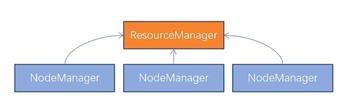
\includegraphics[width=\linewidth]{YARN_architecture.jpg}
    \captionof{figure}{YARN Architecture}
    \label{fig:yarn_architecture}



\begin{itemize}
    \item \textbf{ResourceManager} centralizes the management of resources and handles the allocation across the cluster.
    \item \textbf{NodeManagers} control the execution of tasks on individual nodes.
    \item \textbf{ProxyServer} routes requests to the ResourceManager.
    \item \textbf{JobHistoryServer} maintains records of job specifics for historical analysis.
\end{itemize}

Node1 is configured as table \ref{tab:yarn_roles} to host the ResourceManager along with the NodeManager, ProxyServer, and JobHistoryServer, enabling centralized control and management of cluster resources. Node2 and Node3 are configured as NodeManagers to handle local job executions as depicted below:

\begin{center}
    \begin{tabularx}{\columnwidth}{|c|X|}
    \hline
    Node & Roles \\
    \hline
    node1 & ResourceManager, NodeManager,
            ProxyServer, JobHistoryServer \\
    node2 & NodeManager \\
    node3 & NodeManager \\
    \hline
    \end{tabularx}
    \captionof{table}{YARN roles across the nodes}
    \label{tab:yarn_roles}
\end{center}

To ensure all configurations are effective, necessary configuration files are distributed and maintained:
\begin{itemize}
    \item \textbf{mapred-env.sh, mapred-site.xml} - Configure MapReduce environments and specify the execution framework.
    \item \textbf{yarn-env.sh, yarn-site.xml} - Set up environmental variables and configurations specific to YARN operations.
\end{itemize}

Commands used to initialize and manage the YARN services include:

\begin{lstlisting}
    start-yarn.sh
    mapred --daemon start historyserver
\end{lstlisting}

These steps are crucial for starting the YARN cluster services and ensuring that the ResourceManager and NodeManagers are operational. The status and health of the YARN can be monitored via the web interface accessible at \texttt{node1:8088}.


\subsection{Dataset Preparation}
\subsubsection{Data Collection}
All datasets utilized in this study are sourced from Kaggle, ensuring a comprehensive and diverse representation of AI-related job salaries, which span a wide range of fields including AI, Machine Learning, and Big Data. The selection criteria for the datasets included relevance to the job market, data completeness, and the time frame from 2020 to 2024. This ensures that the data are not only comprehensive but also contemporary and reflective of current trends in technology employment \cite{jahid2024global, aijobs2024global, felinto2024eda, zangari2024jobs}.



\subsubsection{Data Processing}
The data collected from Kaggle underwent rigorous preprocessing steps using Scikit-Learn to ensure their suitability for analysis. The preprocessing steps included data cleaning, where missing values were addressed and anomalies were removed. Data normalization was performed to bring all data features onto a similar scale, thereby preventing any one feature from disproportionately influencing the predictive model due to its scale. Additionally, transformation processes were applied to convert raw data into a format more suitable for analysis. This included converting categorical data into numerical formats and creating new composite features that might be more predictive of the outcomes being modeled. The results after data cleaning and preprocessing are shown in the table \ref{tab:preprocessed_data}.

\begin{table*}[htbp]
    \centering
    \small
    \setlength{\tabcolsep}{0.3pt} % 缩小列间距
    \renewcommand{\arraystretch}{0.9} % 增加行高
    \begin{tabular}{|c|c|c|c|c|c|}
    \hline
    \textbf{work\_year} & \textbf{experience\_level} & \textbf{employment\_type} & \textbf{company\_size} & \textbf{job\_title\_encoded} & \textbf{salary\_in\_usd} \\
    \hline
    2024 & SE & FT & M & 74 & 170955 \\
    2024 & SE & FT & M & 74 & 130270 \\
    2024 & MI & FT & M & 150 & 92144 \\
    2024 & MI & FT & M & 150 & 57616 \\
    2024 & SE & FT & M & 155 & 201600 \\
    \hline
    \end{tabular}
    \caption{Preprocessed Data\textbf{(head)}}
    \label{tab:preprocessed_data}
    \smallskip % 添加少量间距后写注释
    \small
    \textbf{Notes:}
    \begin{itemize}
        \centering
        \item \textbf{SE}: Senior Level
        \item \textbf{MI}: Mid Level
        \item \textbf{FT}: Full Time
        \item \textbf{M}: Medium Company Size
    \end{itemize}
\end{table*}
    
    
    

\section{Methods}
\subsection{Using sklearn and LightGBM for Feature Importance and Model Selection}

\subsubsection{Feature Importance Ranking}
Feature importance in machine learning models is crucial for understanding the factors driving predictions, particularly in models predicting AI job salaries. In this work, I leverage the random forest algorithm from \texttt{scikit-learn}, which inherently computes feature importances for regression tasks. 

In \texttt{RandomForestRegressor}, each tree in the ensemble is trained on a bootstrapped subset of data. The impurity decrease (based on Mean Squared Error in regression) associated with each split is accumulated for each feature across all trees. This total decrease is then normalized to provide a feature importance score, allowing us to rank features by their predictive impact.

The Mean Squared Error (MSE), commonly used to measure impurity for regression, is defined as:
\[
\text{MSE} = \frac{1}{n} \sum_{i=1}^{n} (y_i - \hat{y}_i)^2
\]
where \(y_i\) are the actual target values and \(\hat{y}_i\) are the model predictions. Features that lead to larger reductions in MSE across splits and trees are deemed more important.

Figure~\ref{fig:feature_importance} shows the resulting feature importances from our random forest model, illustrating which variables most strongly influence salary predictions.

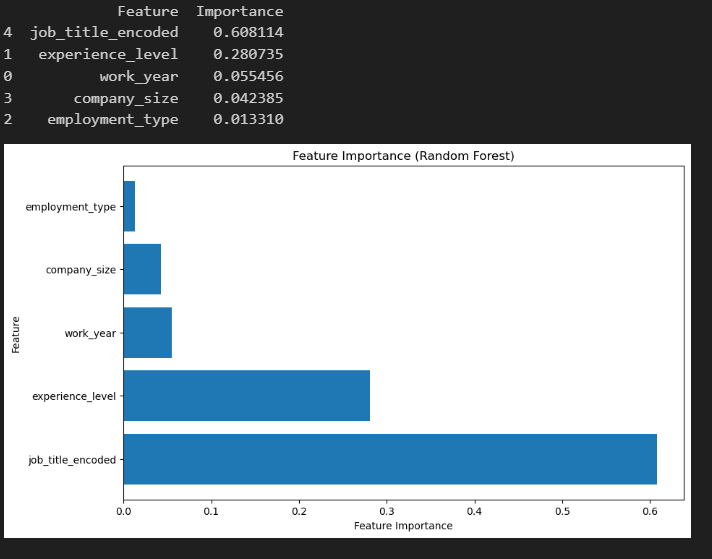
\includegraphics[width=\linewidth]{feature_importance.jpg}
\captionof{figure}{Feature Importance}
\label{fig:feature_importance}

\subsubsection{Model Selection}
Selecting an appropriate machine learning model is essential for achieving high predictive accuracy in AI job salary prediction. I evaluate three commonly used regression models:

\begin{itemize}
    \item \textbf{Random Forest (RF)}
    \item \textbf{LightGBM}
    \item \textbf{Linear Regression}
\end{itemize}

In all models, I apply a logarithmic transformation to the salary variable to mitigate skewness and stabilize variance, i.e., I train on \(\log(1 + \text{salary})\) and invert predictions with \(\exp(\cdot) - 1\).

\paragraph{Random Forest Regressor} 
Random Forest combines multiple decision trees, each trained on different subsamples of the data and features, to reduce overfitting and variance. I initialize the model with:
\begin{lstlisting}
rf_model = RandomForestRegressor(
    random_state=42, 
    n_jobs=3  # Parallelization or serial running
)
rf_model.fit(X_train, y_train)
\end{lstlisting}
I then predict on the test set and compute error metrics such as MSE, MAE, and \(R^2\). Alongside predictions, the model also produces a feature importance ranking.

\paragraph{LightGBM Regressor}
LightGBM is a gradient boosting framework that builds an ensemble of decision trees in a stage-wise fashion, focusing on reducing residual errors at each step. I demonstrate both a default configuration and a hyperparameter-tuned version using \texttt{GridSearchCV}:

\begin{lstlisting}
lgb_model = lgb.LGBMRegressor(random_state=42)
lgb_model.fit(X_train, y_train)  # default training

# hyperparmeter optimization
param_grid = {
    "num_leaves": [31, 63, 127],
    "learning_rate": [0.01, 0.05, 0.1],
    "n_estimators": [100, 200, 300]
}

grid_search = GridSearchCV(
    estimator=lgb.LGBMRegressor(random_state=42),
    param_grid=param_grid,
    cv=3,
    scoring="r2",
    n_jobs=-1   # i cannot use this model for Benchmark
)
grid_search.fit(X_train, y_train)
best_lgb = grid_search.best_estimator_
\end{lstlisting}
LightGBM is known for its speed and accuracy, but it requires careful tuning of \texttt{num\_leaves}, \texttt{learning\_rate}, and \texttt{n\_estimators} to avoid overfitting and ensure good generalization.

\paragraph{Linear Regression}
Linear Regression serves as a simpler baseline model to benchmark the performance of more complex ensemble methods. I use the standard \texttt{LinearRegression} class from \texttt{scikit-learn}:

\begin{lstlisting}
lr_model = LinearRegression(n_jobs=1) # here i can choose how many CPUs
lr_model.fit(X_train, y_train)
\end{lstlisting}
While linear regression provides quick training and interpretability via model coefficients, it may not capture non-linearities in the data.
This is also reflected in the subsequent results discussion.
\subsubsection{Comparison and Selection Strategy}
I compare all models using the MSE, MAE, and \(R^2\) on the test set:
\begin{equation}
    \begin{aligned}
    \text{MSE} &= \frac{1}{n}\sum_{i=1}^{n}(y_i - \hat{y}_i)^2,\\
    \text{MAE} &= \frac{1}{n}\sum_{i=1}^{n}\lvert y_i - \hat{y}_i\rvert,\\
    R^2 &= 1 - \frac{\sum_{i=1}^{n}(y_i - \hat{y}_i)^2}{\sum_{i=1}^{n}(y_i - \bar{y})^2},
    \end{aligned}
    \label{MSE_MAE_R}
\end{equation}
    
in equation \eqref{MSE_MAE_R} where \(y_i\) are the actual salary values (in the original scale after inverse-log transform), \(\hat{y}_i\) are predictions, and \(\bar{y}\) is the mean of the actual values.

The Random Forest and LightGBM models both exhibit strong performance, with LightGBM typically providing faster convergence and slightly higher accuracy when optimized. Linear Regression, although simpler, remains a useful baseline and offers interpretability of feature coefficients. Ultimately, I select an optimized LightGBM for final deployment due to its balance of speed, accuracy, and robust hyperparameter tuning. 

\subsection{Parallel Model Fitting using PySpark and Hadoop}

When dealing with large-scale datasets, training machine learning models in a distributed computing environment is crucial. In this study, I employ Apache Spark's MLlib library to parallelize model training across a Hadoop YARN cluster. The process involves setting up a SparkSession, feature engineering, and model training using multiple regression algorithms.

\subsubsection{Initializing SparkSession in Hadoop Cluster}

To leverage Spark's distributed computing capabilities, I first initialize a \texttt{SparkSession}, which serves as the entry point for Spark applications. Since I operate on a Hadoop cluster, the session is configured to run in \texttt{yarn} mode, enabling resource allocation across cluster nodes. The initialization is performed as follows:

\begin{lstlisting}
from pyspark.sql import SparkSession

spark = SparkSession.builder \
    .appName("SalaryPrediction") \
    .config("spark.sql.shuffle.partitions", "200") \
    .config("spark.executor.memory", "4g") \
    .config("spark.driver.memory", "4g") \
    .config("spark.executor.cores", "2") \
    .config("spark.executor.instances", "3") \
    .master("yarn") \
    .getOrCreate()
\end{lstlisting}

\begin{itemize}
    \item \textbf{appName}: Sets the application name for tracking in Spark UI.
    \item \textbf{spark.sql.shuffle.partitions}: Defines the number of partitions used for shuffling data during operations like joins.
    \item \textbf{spark.executor.memory}: Allocates memory per executor, ensuring efficient resource usage.
    \item \textbf{spark.executor.instances}: Specifies the number of executor instances across the Hadoop cluster.
    \item \textbf{master("yarn")}: Enables Spark to run in a distributed mode using Hadoop YARN.
\end{itemize}

\subsubsection{Feature Engineering with Spark MLlib}
Once the session is initialized, feature engineering is performed using Spark's built-in transformations. Given that our dataset contains categorical variables such as \texttt{experience\_level} and \texttt{employment\_type}, I apply encoding techniques to convert them into numerical representations.

\begin{lstlisting}
from pyspark.ml.feature import StringIndexer, OneHotEncoder, VectorAssembler

# Encoding categorical variables
indexers = [
    StringIndexer(inputCol=col, outputCol=f"{col}_index")
    for col in ["experience_level", "employment_type", "company_size", "job_title"]
]

encoder = OneHotEncoder(
    inputCols=[f"{col}_index" for col in ["experience_level", "employment_type", "company_size", "job_title"]],
    outputCols=[f"{col}_vec" for col in ["experience_level", "employment_type", "company_size", "job_title"]]
)

# Assembling feature vectors
assembler = VectorAssembler(
    inputCols=["work_year", "experience_level_vec", "employment_type_vec", "company_size_vec", "job_title_vec"],
    outputCol="features"
)
\end{lstlisting}

\subsubsection{Training Models in Parallel}
With the features prepared, I train multiple regression models in parallel using Spark MLlib. The models include:

\begin{itemize}
    \item \textbf{Linear Regression (LR)}: A simple yet effective baseline model.
    \item \textbf{Random Forest Regressor (RF)}: An ensemble model that constructs multiple decision trees.
    \item \textbf{Gradient Boosted Trees (GBT)}: A boosting method that sequentially improves weak models.
\end{itemize}

The models are initialized and trained using the following Spark MLlib methods:

\begin{lstlisting}
from pyspark.ml.regression import LinearRegression, RandomForestRegressor, GBTRegressor

# Define models
lr = LinearRegression(featuresCol="features", labelCol="salary_in_usd", maxIter=50, regParam=0.1)
rf = RandomForestRegressor(featuresCol="features", labelCol="salary_in_usd", numTrees=100)
gbt = GBTRegressor(featuresCol="features", labelCol="salary_in_usd", maxIter=50)

# Fit models in parallel
models = {"Linear Regression": lr, "Random Forest": rf, "GBT": gbt}
trained_models = {name: model.fit(training_data) for name, model in models.items()}
\end{lstlisting}


\section{Results}
\subsection{Experimental Results}
This section provides a detailed evaluation of the models' performances based on accuracy metrics and validation results. The evaluation includes a comparative analysis of error metrics, highlighting the challenges encountered in predicting AI job salaries.

Despite using various machine learning models in sklearn and experimenting with different data filtering techniques, the models did not achieve satisfactory performance. The overall fit was poor, as reflected in the high error values. The reasons behind this could be manifold.

One possible explanation is that the imputation of missing values during data preprocessing may have introduced noise, making it difficult for the models to extract meaningful patterns. Another potential reason is the inherent variability in AI job salaries, where different positions have significantly different compensation levels, leading to a high degree of salary dispersion. These factors could have contributed to the difficulty in fitting the data effectively.

The following figure \ref{fig:Error_results} presents a comparison of error metrics, including RMSE and MAE, for different models, illustrating their respective performance discrepancies.

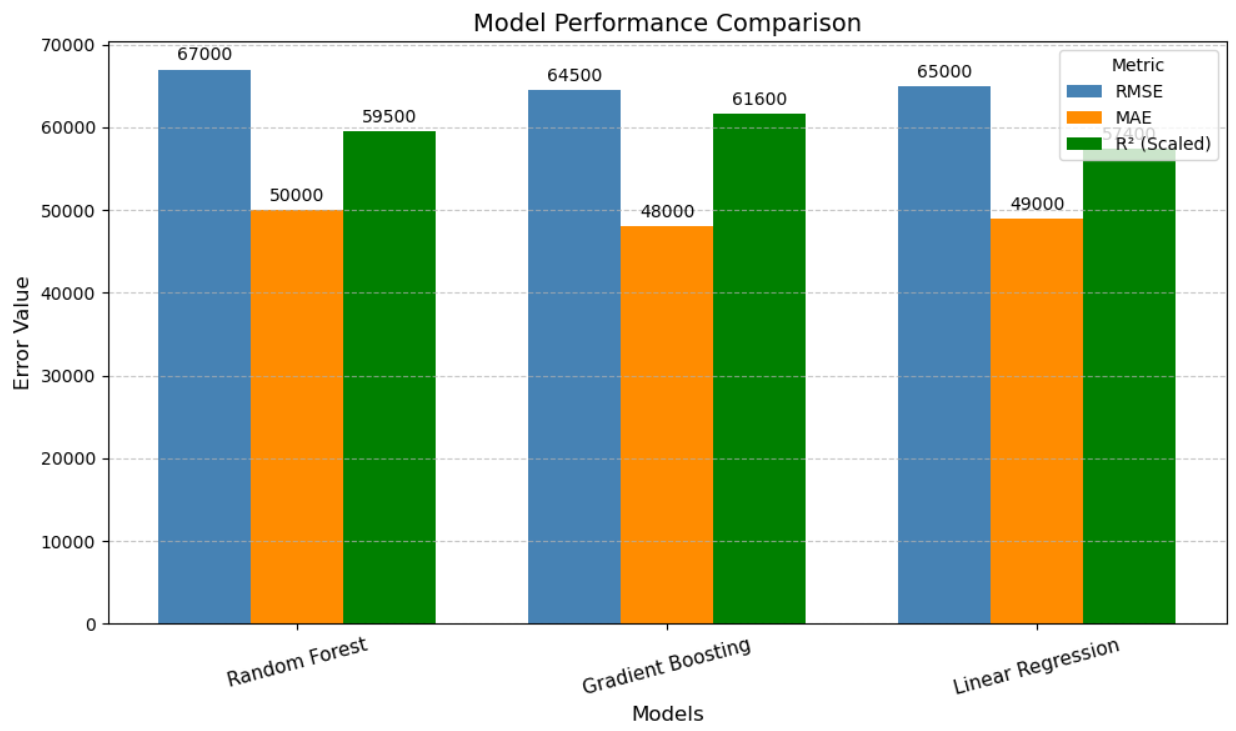
\includegraphics[width=\linewidth]{error_result.jpg}
\captionof{figure}{Comparison of Error Results}
\label{fig:Error_results}

Additionally, the figure \ref{fig:prediction_results} below displays the predicted salary values compared to actual salaries. The inconsistency between predicted and true values further highlights the challenge of accurately modeling AI job salaries.

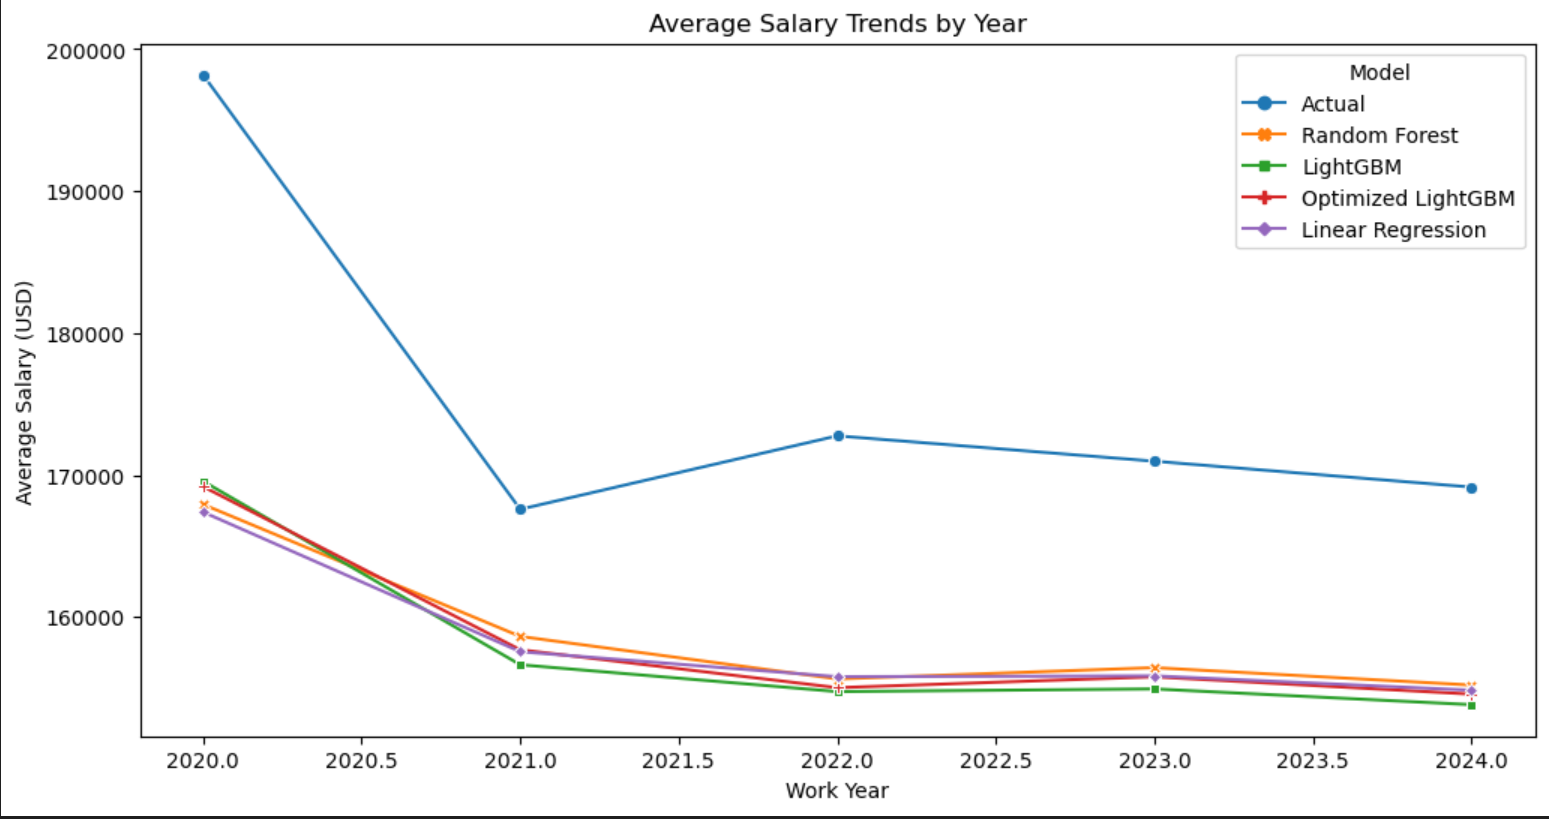
\includegraphics[width=\linewidth]{prediction_result.jpg}
\captionof{figure}{Prediction Results}
\label{fig:prediction_results}

\subsection{Benchmark}
Evaluating the performance of machine learning frameworks is crucial, especially when dealing with large-scale data. In this section, I compare the execution times of machine learning models trained using \textbf{scikit-learn (sklearn)} and \textbf{PySpark} within a Hadoop cluster. The benchmark focuses on two models: \textbf{Random Forest} and \textbf{Linear Regression}, assessing how well they scale across different computing environments.

\textbf{Performance Comparison:}  
The benchmark compares three scenarios:
\begin{enumerate}
    \item Training with \textbf{scikit-learn} on a single CPU.
    \item Training with \textbf{scikit-learn} using parallelization across three CPUs.
    \item Training with \textbf{PySpark} on a Hadoop cluster(with 3 nodes, 3 CPUs).
\end{enumerate}

The results, visualized in Figure~\ref{fig:Benchmark}, show a significant performance improvement when using PySpark, particularly in the case of the Random Forest model. The execution time for Random Forest with PySpark is considerably lower than that of scikit-learn, even when sklearn utilizes multiple CPUs. Similarly, the Linear Regression model also benefits from the distributed computing environment, albeit to a lesser extent.

\textbf{Key Observations:}  
\begin{itemize}
    \item The Random Forest model exhibits the most notable speedup, reducing training time dramatically when run on the Hadoop cluster.
    \item Even for a computationally less expensive model like Linear Regression, PySpark demonstrates an efficiency advantage over scikit-learn.
    \item The impact of using multiple CPUs in scikit-learn is noticeable but still falls behind PySpark's distributed computing approach.
    \item Despite the relatively low hardware specifications of the Hadoop cluster used in this study, the acceleration is substantial.
\end{itemize}

This benchmark highlights the effectiveness of \textbf{Hadoop and PySpark} in accelerating machine learning workloads, making them a viable solution for large-scale predictive modeling tasks.

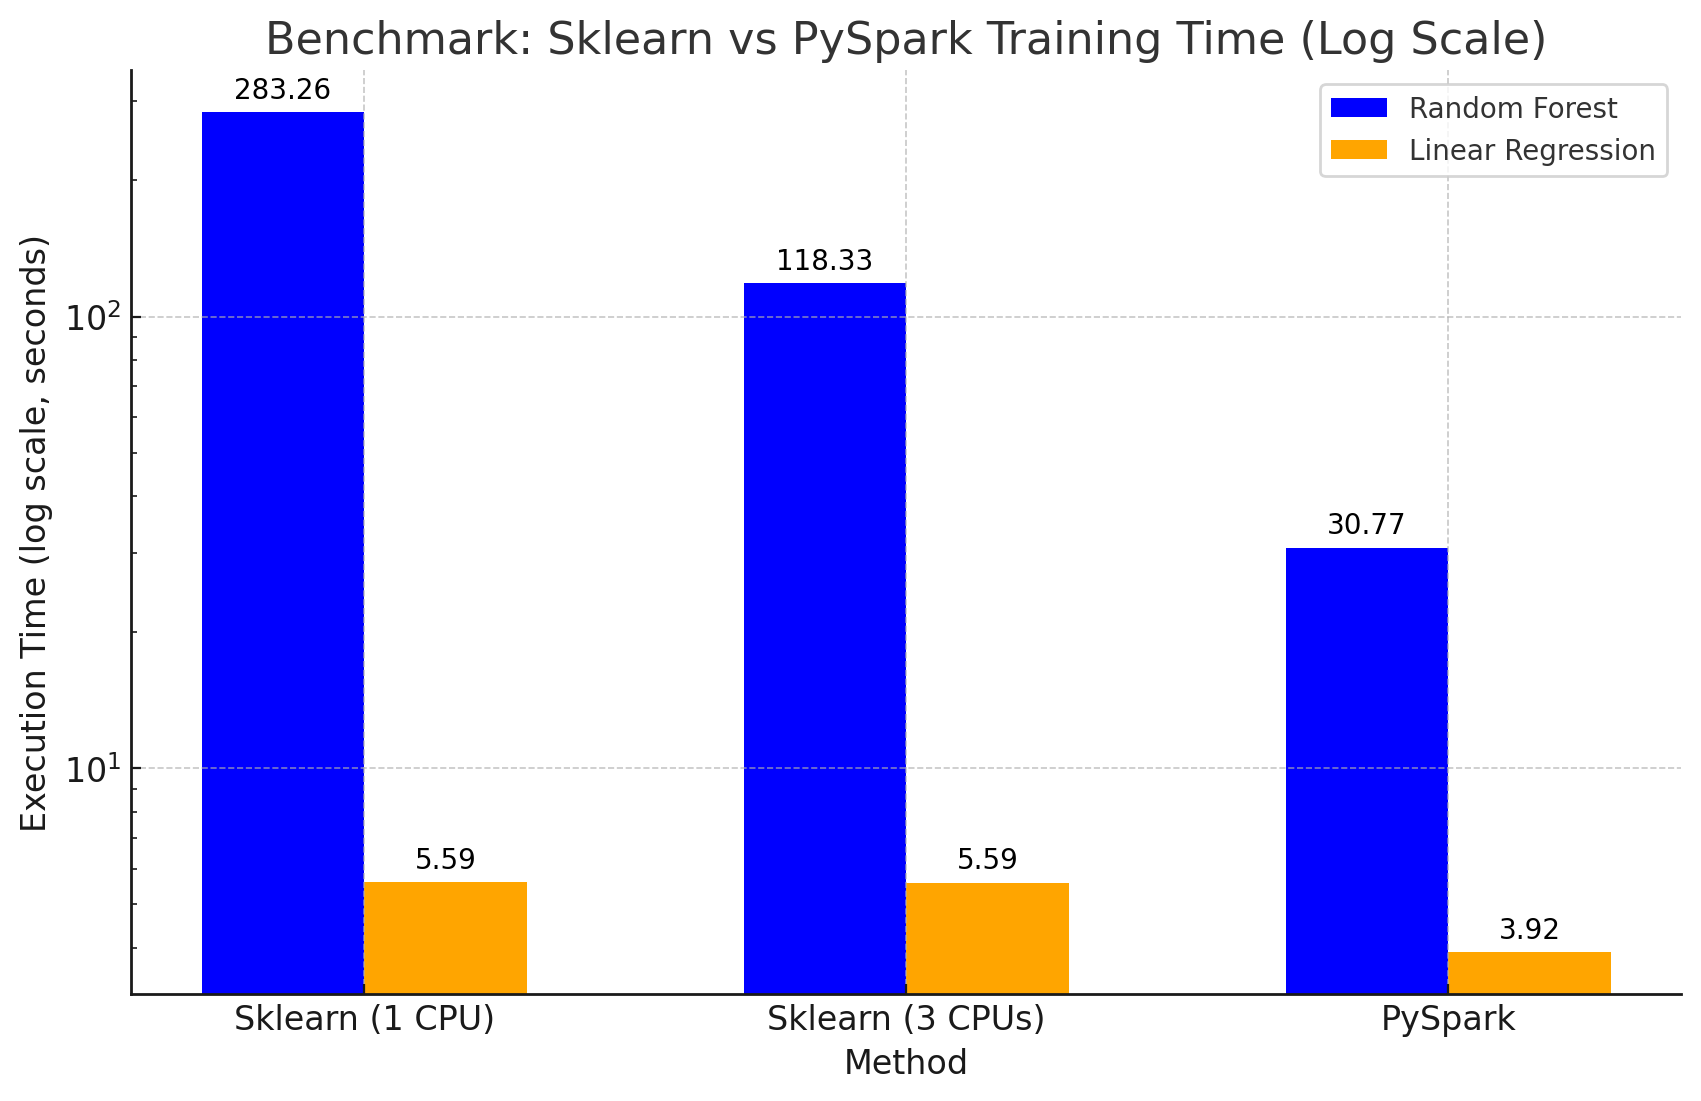
\includegraphics[width=\linewidth]{Benchmark.png}
\captionof{figure}{Benchmark of sklearn and PySpark}
\label{fig:Benchmark}

Although Spark significantly accelerates model training, based on the performance evaluation steps, I did not include the time required to upload the dataset to the HDFS cluster in the total computation time. In real-world scenarios, the dataset size may be significantly larger than the one I collected, meaning that the time required for data transfer and storage in HDFS could be substantially higher. This additional overhead should be taken into account when evaluating the overall efficiency of a distributed training pipeline.
\subsection{Literature-Based Findings}

The integration of AI into the workforce has been expanding at an unprecedented rate, with significant implications for job roles, compensation, and professional development. Several reports provide insights into these trends, highlighting both opportunities and challenges.
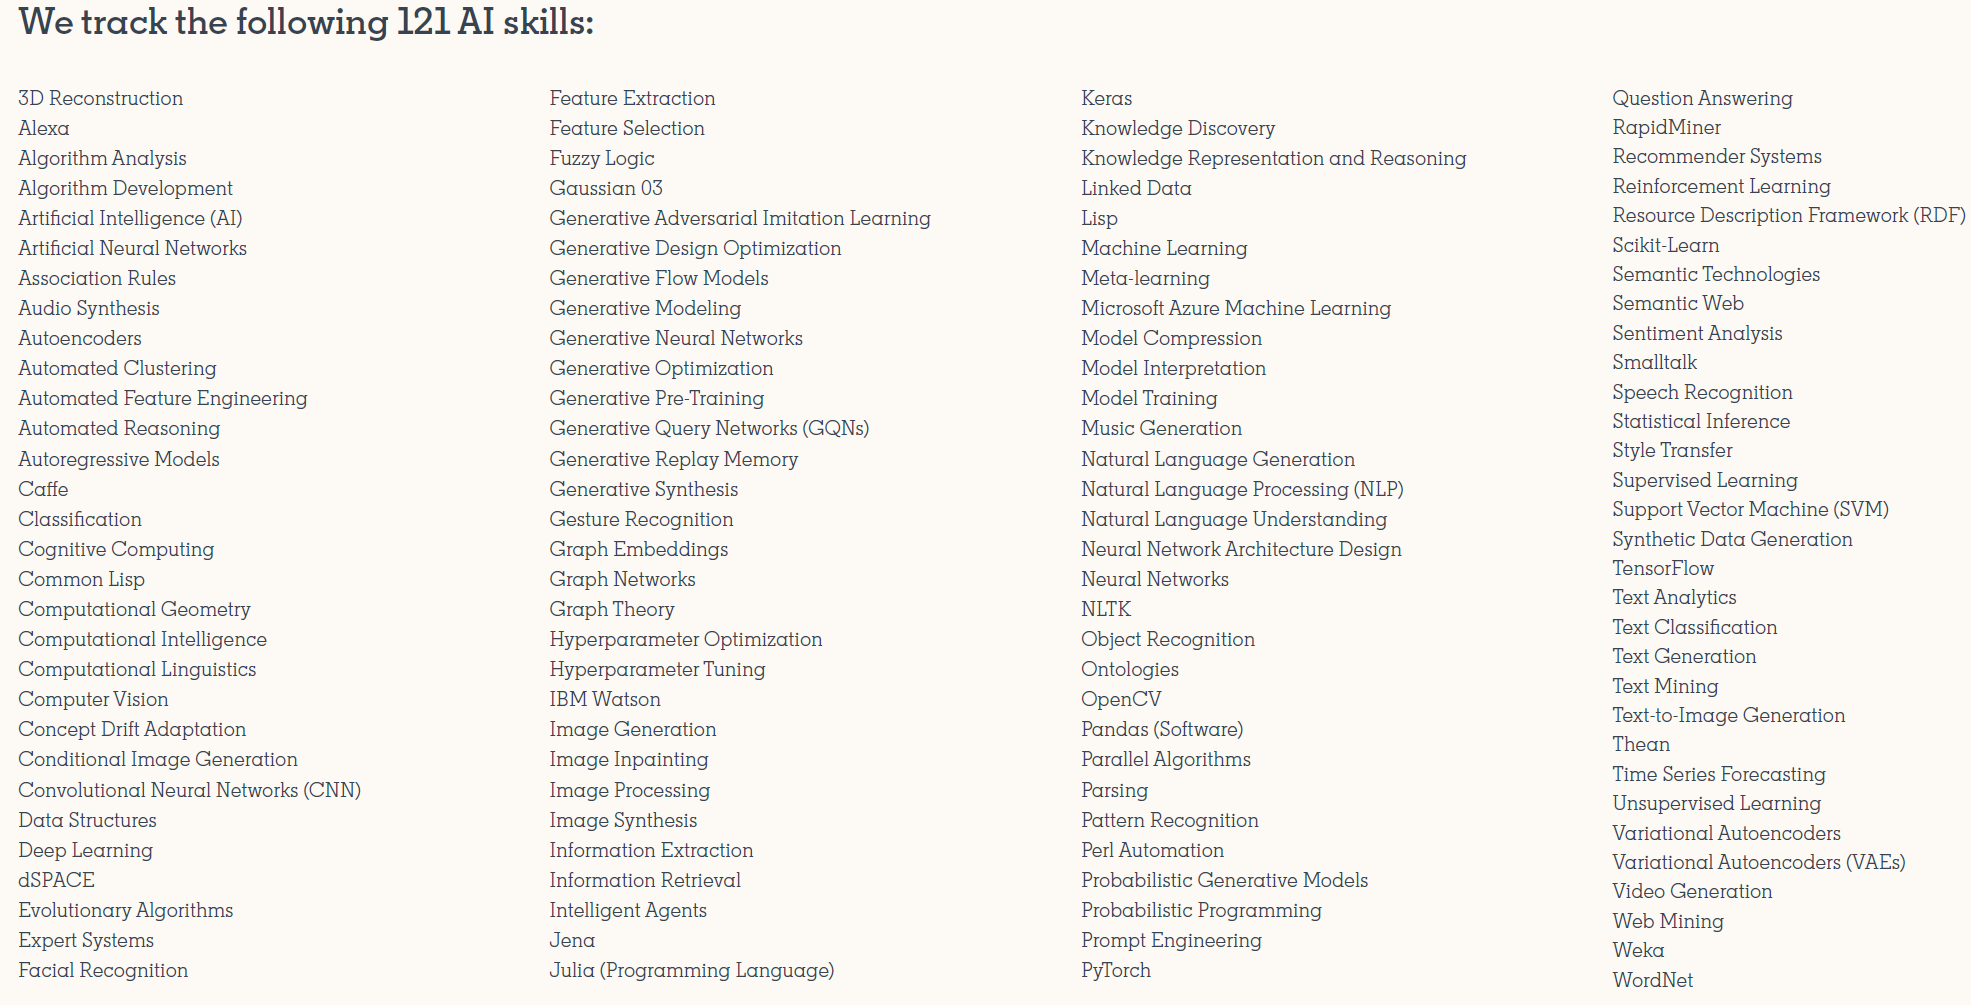
\includegraphics[width=\linewidth]{AI_skills.jpg}
\caption{AI-related skills}
\label{fig:AI_skills}

Given that the final results of my project do not accurately reflect the real-world trends in AI salaries in the United States, I have also gathered and analyzed a selection of published reports that have already conducted comprehensive statistical assessments. By incorporating these established datasets, I aim to compare my findings with verified salary trends, thereby gaining a more accurate understanding of the actual state of AI compensation and identifying potential discrepancies in my analysis.
\cite{linkedin2023future} reports that as of June 2023, the number of professionals with AI-related skills had increased ninefold since January 2016, reflecting a substantial global shift toward AI proficiency. This rapid expansion suggests that AI-related expertise is becoming a fundamental requirement across multiple industries.

Furthermore, generational perspectives on AI adoption indicate a strong optimism among younger professionals. According to \cite{linkedin2023future}, 52\% of Millennials and 48\% of Gen Z professionals believe that AI will positively impact their career trajectories by offering faster access to knowledge and insights. This demonstrates a growing confidence in AI as an enabler of career advancement, particularly among digital-native generations.

In addition to the widespread adoption of AI skills, the job market is witnessing increasing specialization within the field. \cite{wids2024salary} identifies the emergence of distinct AI-focused roles such as AI Engineer, Prompt Engineer, NLP Specialist, and Computer Vision Engineer. This trend underscores the industry's shift toward more nuanced and highly technical AI roles, which require deep expertise in machine learning, data processing, and algorithm development.

From a compensation perspective, salaries for AI and data science professionals have shown dynamic trends over the past few years. \cite{wids2024salary} notes that after a significant increase in 2022, salaries for AI and data science professionals have now stabilized, suggesting a maturation of the job market. This stabilization may be attributed to a more balanced supply-demand dynamic as more professionals acquire AI expertise.

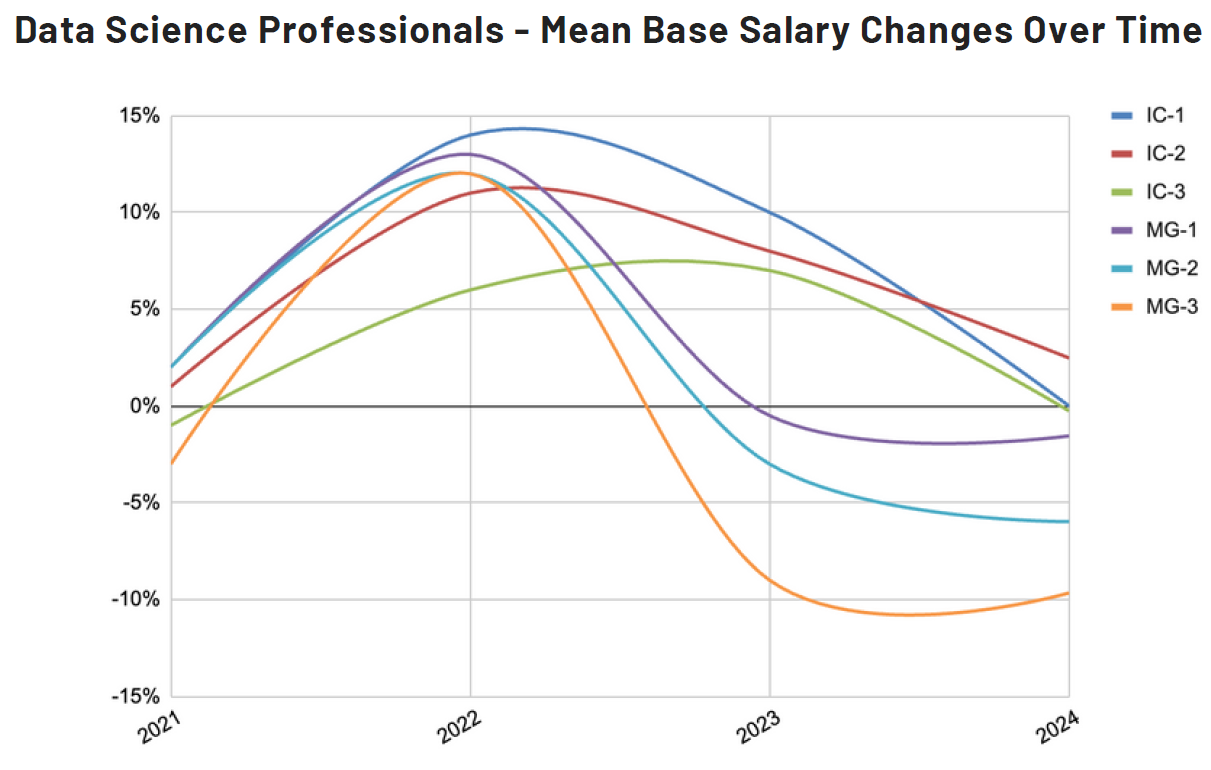
\includegraphics[width=\linewidth]{Data_Scientist_Salary.jpg}
\captionof{figure}{Data Science Professionals - Mean Base Salary Changes Over Time\raisebox{1ex}{\cite{wids2024salary}}.}
\label{fig:Data_Scientist}

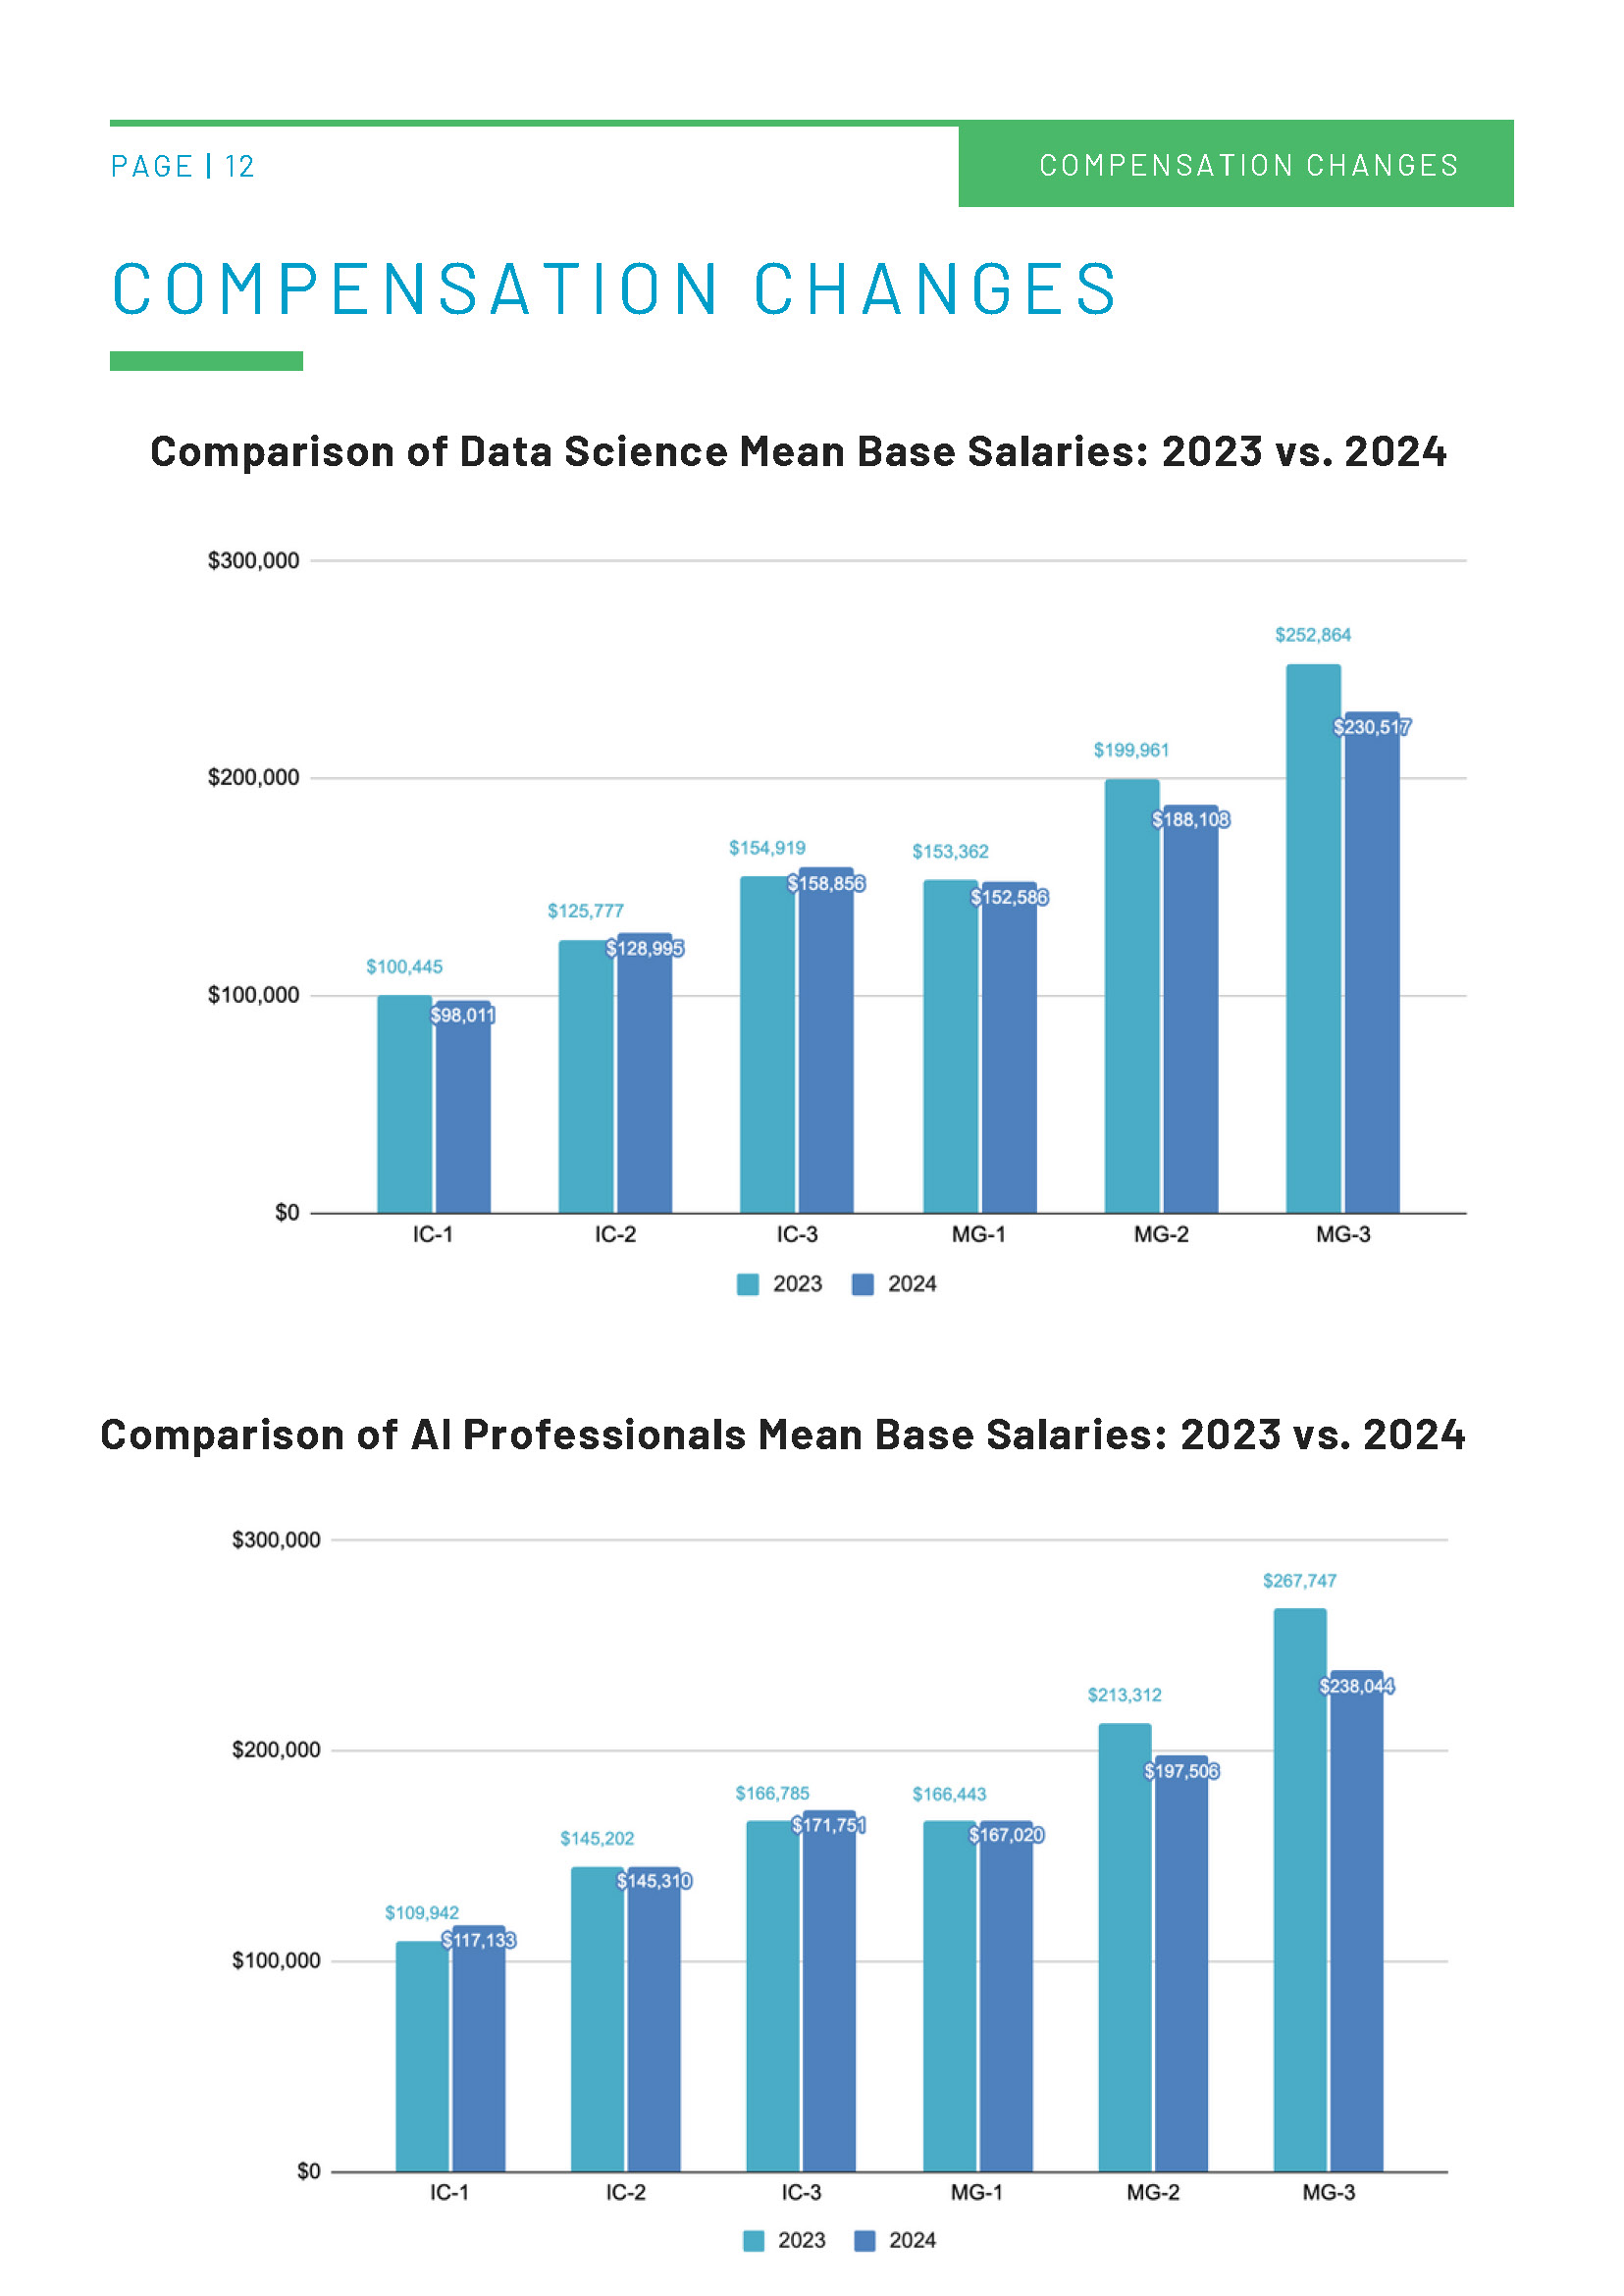
\includegraphics[scale=0.3]{Comparision_Changes.jpg}
\captionof{figure}{Comparison of Data Science \& AI Professionals Mean Base Salaries: 2023 vs 2024\raisebox{1ex}{\cite{wids2024salary}}.}
\label{fig:Comparision_Changes}

Despite the enthusiasm surrounding AI's potential, the transformation of the workplace is still in its early stages. \cite{linkedin2023future} emphasizes that "we have only just begun to understand the potential for AI to transform the way we work, the way we learn, and the way we interact with others." This sentiment reflects the ongoing evolution of AI applications, which continue to reshape industries, redefine job roles, and introduce new ethical and operational challenges.
\
Collectively, these findings illustrate the expanding influence of AI across industries, the increasing demand for specialized roles, the stabilization of AI-related compensation, and the shifting attitudes toward AI among professionals. As AI technology continues to evolve, its long-term impact on employment structures, career development, and workforce dynamics remains a critical area of study.

\section{Conclusion}

This project was a unique experience, as I successfully set up a fully functional Hadoop cluster and YARN system on a notebook with minimal configuration. Throughout the process, I gained a comprehensive understanding of the inner workings of a Hadoop cluster, the execution of MapReduce jobs, and the system workflow as reflected in the final job reports. This journey from zero to one was both challenging and rewarding. However, the project was not without its limitations, and several areas remain for improvement.

\subsection{Limitations of the Study}

Despite my initial confidence in setting up a small-scale HDFS and YARN system, I encountered significant challenges during the early stages of the project. The preliminary setup and configuration process took considerably longer than expected, requiring extensive trial and error, debugging, and optimization. This unforeseen delay had a cascading effect on the later stages of the project, particularly in the data processing and model evaluation phase.

Due to the time constraints imposed by the prolonged system setup, I was unable to allocate sufficient resources for experimenting with different data preprocessing techniques and model tuning strategies. This limitation was particularly evident in the comparative analysis using PySpark and Scikit-learn, where the lack of iteration and refinement led to suboptimal model performance. Ultimately, the final model fitting results were unsatisfactory, failing to meet the intended objectives of the study. A more structured time management approach and contingency planning for unexpected delays could have mitigated these challenges.

\subsection{Future Work}

Moving forward, my focus will not only be on gaining a deeper understanding of system workflows and operational principles but also on achieving verifiable results and measurable outcomes. Understanding the theoretical aspects of big data processing and AI model development is essential, but the ability to apply these tools effectively and obtain meaningful insights is equally, if not more, important. 

To enhance the effectiveness of future projects, I aim to implement more rigorous planning and validation methodologies, ensuring that system setup and configuration do not impede critical analytical tasks. Additionally, I will prioritize the development of robust models with well-defined evaluation metrics, allowing for concrete assessment and comparison of results. By refining these aspects, I hope to bridge the gap between theoretical knowledge and practical application, ultimately improving my proficiency in big data processing and AI-driven analytics.

\end{multicols}

% \begin{multicols}{2}
\bibliographystyle{plain}
\bibliography{reference}
% \end{multicols}

\end{document}
